        \title[\whatshort, \simplenum, 
Slide \insertframenumber/\inserttotalframenumber ] {\what}
% this dirty hack allows me to display frame numbers in the footnotebar.

 

\subtitle{Class \simplenum: Reinforcement Learning}



\usepackage{graphicx}
%\subtitle{}

\begin{document}

\begin{frame}
  \titlepage

\end{frame}

\begin{frame}
  \frametitle{Class Outline} \tableofcontents % You might wish to add
  %the option [pausesections]
\end{frame}


% Since this a solution template for a generic talk, very little can
% be said about how it should be structured. However, the talk length
% of between 15min and 45min and the theme suggest that you stick to
% the following rules:  

% - Exactly two or three sections (other than the summary).
% - At *most* three subsections per section.
% - Talk about 30s to 2min per frame. So there should be between about
%   15 and 30 frames, all told.

\begin{frame}[fragile]
\frametitle{References}

\begin{itemize}

\item[[TM{]}] T.~M.~Mitchell, ``Machine Learning'', McGraw-Hill, 1998,
  Chapter 13.

\item[[SB{]}] R.~S.~Sutton and A.~G.~Barto, 
``Reinforcement Learning: An Introduction'', 2nd edition, The MIT
Press, 2018

\item[[CS{]}]  C.~Szepesv\'ari
``Algorithms for Reinforcement Learning'', Morgan \& Claypool, 2010

\item[[JT{]}] J.~N.~Tsitsiklis, On the Convergence of Optimistic Policy
Iteration, JMLR 3 (2002) 59-72

\item[[WD{]}] C.~J.~C.~H.~Watkins and P.~Dayan, Technical Note:
Q-Learning, Machine Learning, 8, 279-292 (1992)

\end{itemize}
\end{frame}

\section[Preliminaries]{Environment and Policy}

\begin{frame}\frametitle{Principal Setup}

\begin{itemize}

\item a learning agent interacts with an environment

--- the agent takes an action

--- the environment gives a reward and changes its state

\bigskip

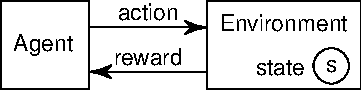
\includegraphics[scale=1]{agent_environment}

\item we make the Markov assumption: all activity (choice of the
action, reward, state to go to) depends on the
current state rather then the whole history

--- given the current state, the future is independent of the past

\item the current state is visible to the agent

\end{itemize}
\end{frame}


\begin{frame}\frametitle{Gridworlds}
\begin{itemize}

\item gridworlds are toy examples used to illustrate principles of
reinforcement learning

\bigskip

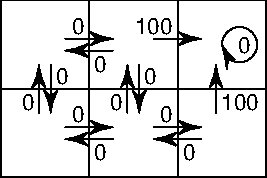
\includegraphics[scale=1]{gridworld}
\begin{minipage}{5cm}
~~~~~~~~~~~~(after [TM], Fig.~13.2)
\end{minipage}

\item the agent can move from a square to a neighbouring square; the
rewards are shown on the diagram

\item here the top right corner is a \alert{goal state (or terminal
state)}; further moves from it are neither possible nor needed

\end{itemize}
\end{frame}

\begin{frame}\frametitle{Deterministic Environment}
\begin{itemize}

\item this example is a deterministic environment

--- the reward and the state we move into are functions of the current
    state and action taken

\item let $S$ be the set of all states and $A$ be the set of all
    actions; if the environment is deterministic, then


--- reward $r = \text{Reward}(s,a)$, where $\text{Reward}: S\times
    A\to \R$ is a function

--- state we move into $s = \text{State}(s,a)$, where $\text{State}:
    S\times A\to S$ is a function

\item the environment can be described by two functions

\end{itemize}
\end{frame}

\begin{frame}\frametitle{Stochastic Environment}
\begin{itemize}

\item suppose we are controlling a robot in a real-life situation

\item there is uncertainty as to what happens after an action

--- the reward we get and the state we move into after taking an
    action $a$ in a state $s$ can be modelled by random variables
    $\text{Reward}_{s,a}$ and $\text{State}_{s,a}$

\item the environment may be described by a collection of
    distributions on $S\times \R$

--- there is one distribution for each pair $(s,a)$

\item this is called a \alert{Markov Decision Process (MDP)}

\item we assume the MDP is stationary, i.e., if we return to state $s$
and choose the same action $a$, we are faced with the same
probabilities

\end{itemize}
\end{frame}


\begin{frame}\frametitle{Finite MDP}
\begin{itemize}

\item we will be dealing with the case of finite sets of states $S$
and actions $A$

\item an MDP specifies:

--- the probabilities that upon choosing an action
$a$ in a state $s$ we move to a state $s'$: $\Pr(s'\mid s,a)$

--- the random variable $R_{s,a}$ giving us the reward if we choose an
action $a$ in a state $s$

\item we assume that all rewards are bounded

--- more technical assumption: the expectation and variance of
    $R_{s,a}$ exist

\end{itemize}
\end{frame}

\begin{frame}\frametitle{Policy}
\begin{itemize}

\item a deterministic policy is a function from states to actions
    $\pi: S\to A$

--- given a state, it tells us what action we should take

\item a stochastic policy can toss a coin before it decides what
action to take

--- in other words, a stochastic policy is a set of distributions on
    the set of actions, one for each state

\item in the case of a finite MDP, a stochastic policy $\pi$ specifies
    probability $\pi(a\mid s)$ of taking an action $a$ in a state $s$

\end{itemize}
\end{frame}



\section{Value of a State}

\begin{frame}\frametitle{Cumulative Reward}
\begin{itemize}

\item consider an MDA and a policy $\pi$

\item suppose that we start in a state $s_0$ and follow a policy $\pi$

--- we take an action $A_0$ (a random variable), get reward $R_1$ and
    go to the state $S_1$ (both random variables)

--- we then take an action $A_1$, get reward $R_2$ and
    go to the state $S_2$ etc

--- we get a sequence $s_0, A_0, R_1, S_1, A_1, R_2, S_2, A_3,\ldots$ 

\item we want a policy to bring high reward

--- quickly

\item pick a discounting factor $\gamma\in [0,1]$

\item the \alert{discounted cumulative reward} is

$$G_t = R_0 + \gamma R_1 +\gamma^2 R_2 + \gamma^3 R_3+\ldots$$

\end{itemize}
\end{frame}


\begin{frame}\frametitle{Discounting}
\begin{itemize}

\item the choice of $\gamma$ reflects our preferences to immediate
rewards vs future rewards

--- the value $\gamma = 0$ implies that only the immediate reward
    matters

--- the value $\gamma = 1$  implies that the moment of time when the
    reward arrives does not matter at all


\item mathematically the values $\gamma<1$ make sure the series
    converges

--- the sequence of rewards $r_1, r_2, r_3, \ldots$ may be finite (if
    we run into a terminal state, all rewards are zeros from some
    point) or infinite (even if the set of states is finite)

--- but if the rewards are bounded and $\gamma<1$, the series
    $r_0+\gamma r_1+\gamma^2r_2+\ldots$ always converges


\end{itemize}
\end{frame}


\begin{frame}\frametitle{Value of a State}
\begin{itemize}

\item the value

$$V_\pi(s_0) = \bE G_t = \bE ( R_0 + \gamma R_1 +\gamma^2 R_2
+ \gamma^3 R_3+\ldots)$$

shows how much reward $V$ earns on average if we start from state $s_0$

\end{itemize}
\end{frame}


\begin{frame}\frametitle{Optimal Value Function}
\begin{itemize}

\item we want to find an optimal policy maximising rewards

\item define $V^*(s) = \sup_\pi(s)$

--- this is the value of the discounted cumulative reward if we follow
    an optimal policy from $s$

\end{itemize}
\end{frame}


\begin{frame}\frametitle{Gridworld Example}
\begin{itemize}

\item assume $\gamma = 0.9$

\item clearly, the best we can do in the gridworld example is to run
    towards the exit asap

\bigskip

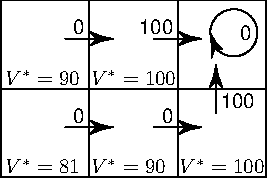
\includegraphics[scale=1]{gridworld_optimal}



\end{itemize}
\end{frame}


\begin{frame}\frametitle{Optimal Policy}
\begin{itemize}

\item we have actually constructed an optimal policy $\pi^*$ such that
$$ V^*(s) = V_{\pi^*}(s)$$

--- our optimal policy achieves the optimal values for all $s$

\item in a general case, is there such a policy?

--- are the values $V^*(s)$ actually achieved by the same $\pi$ for
    different states $s$?

\item we can define an optimal policy as $\pi^*$ such that for any
other policy $\pi$ and any state $s$ we have $V_{\pi^*}(s)\ge
V_{\pi}(s)$

--- does an optimal policy exist?

--- does it achieve $V^*(s)$?

\item the answers to all these questions are positive (at least for
finite MDPs) but this requires further study

\end{itemize}
\end{frame}


\section[DP]{Bellman Equation and Dynamic Programming}

\end{document}










